% !TEX root = ../../main.tex


\begin{figure}[!htbp]
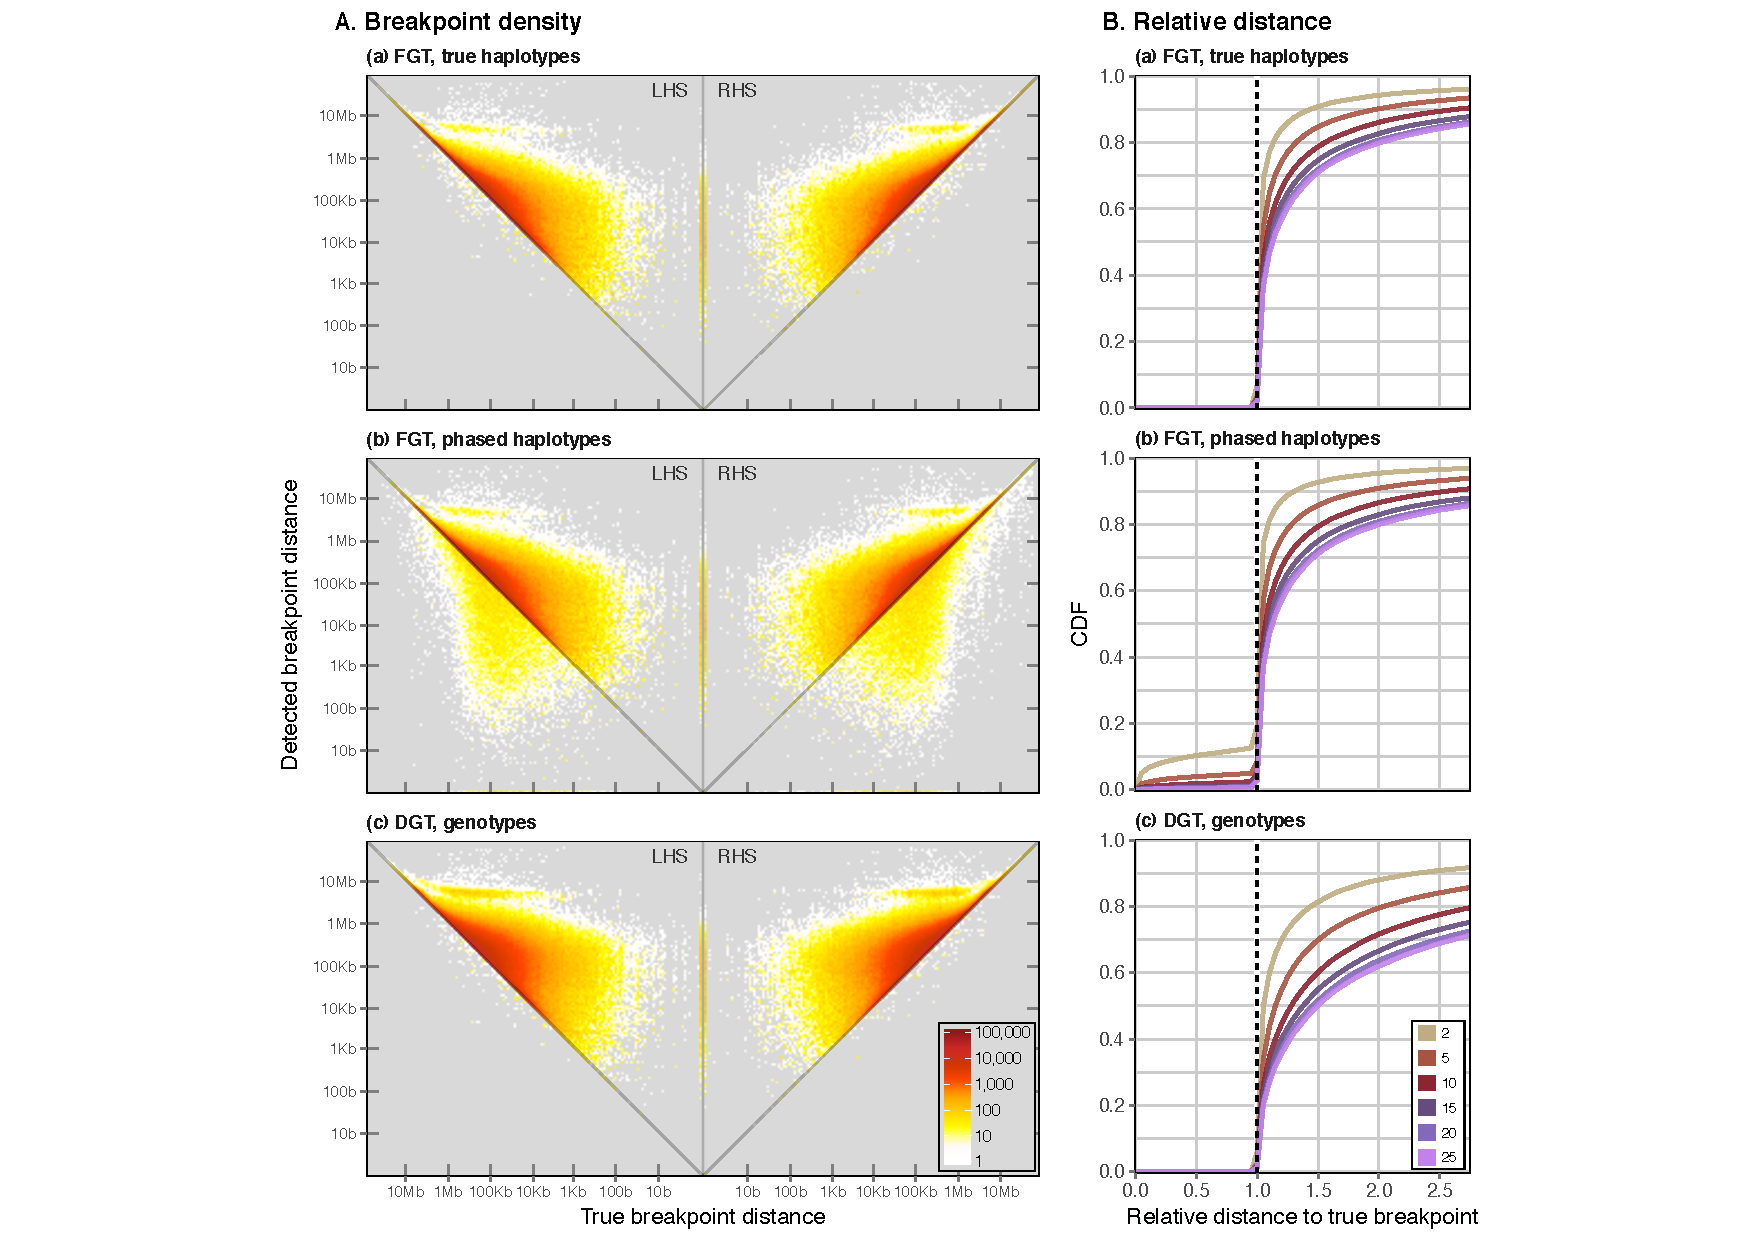
\includegraphics[width=\textwidth]{./img/ch3/naive_break_tru.pdf}
\Caption{Accuracy of breakpoint detection in simulated data}
{Breakpoints detected in \fk{} pairs at ${k \in \lbrace 2, \ldots, 25 \rbrace}$ are compared to true IBD breakpoint sites, after removing boundary cases in either the detected or true dataset.
Segments were inferred using the \gls{fgt} on true haplotypes \textbf{(a)} and phased haplotypes \textbf{(b)}, as well as the \gls{dgt} on genotype data \textbf{(c)}.
Panel~\textbf{(A)} shows the density of detected breakpoints in relative distance to the focal and true breakpoint sites.
The physical distance between detected breakpoint and focal position was divided by the distance between true breakpoint and focal position, such that values $<1$ indicate underestimation and $>1$ overestimation relative to the true distance (\emph{dashed line}).
Panel~\textbf{(B)} illustrates the relationship between each detected breakpoint and the corresponding true breakpoint, measured as the physical distance to the focal site.
Along each axis, distances were pooled into \n{200} bins (on log scale)
and cells in the resulting $200^2$ grid were colour-coded for the number of  intersecting true and detected breakpoints, where grey indicates zero.
Segment breakpoints to the left (\emph{LHS}) and right-and side (\emph{RHS}) of the focal position are shown separately.}
{fig:naive_break_tru}
% \vspace{-5pt}
% \hrulefill
\end{figure}
